% !TEX TS-program = xelatex
% !TEX encoding = UTF-8 Unicode
\documentclass[aspectratio=169]{xmu-slide}

\usepackage{amssymb}
\usepackage{makecell}
\usetikzlibrary{arrows.meta,positioning,shapes.geometric,fit}
\pgfplotsset{compat=1.18}

\title{PipeANN 动态更新实验汇报}
\author{林正刚}
\teacher{沈志荣教授}
\pubdate{}

\setbeamerfont{frametitle}{size=\large,series=\bfseries}

\newcommand{\ok}{\textcolor{green!45!black}{通过}}
\newcommand{\warn}{\textcolor{orange!85!black}{部分通过}}
\newcommand{\bad}{\textcolor{red!75!black}{未达标}}

\begin{document}

\maketitle

\begin{frame}[t]{混合搜索框架}
    \centering
    \scriptsize
    核心目标：同一个索引同时支持低选择性过滤查询和高选择性近似搜索，并为每个查询选择更合适的执行路径。
    \vspace{0.15em}

    \begin{columns}[c,onlytextwidth]
        \column{0.64\textwidth}
        \centering
        \begin{tikzpicture}[
            scale=0.80,
            transform shape,
            font=\scriptsize,
            node distance=0.44cm and 0.48cm,
            box/.style={draw, rounded corners=2pt, align=center, text width=2.35cm, minimum height=0.62cm, fill=blue!5},
            decision/.style={draw, diamond, aspect=1.85, align=center, text width=1.88cm, inner sep=1pt, fill=orange!9},
            route/.style={draw, rounded corners=2pt, align=center, text width=2.75cm, minimum height=0.78cm, fill=green!7},
            data/.style={draw, rounded corners=2pt, align=center, text width=2.42cm, minimum height=0.58cm, fill=gray!8},
            outbox/.style={draw, rounded corners=2pt, align=center, text width=2.30cm, minimum height=0.60cm, fill=purple!6},
            arrow/.style={-{Stealth[length=2mm]}, line width=0.45pt}
        ]
            \node[box] (query) {Query + filter};
            \node[box, below=of query] (selectivity) {选择性估计\\$s=|filter|/N$};
            \node[decision, below=of selectivity] (judge) {$s \leq \tau_m$?};
            \node[route, below left=0.62cm and 0.30cm of judge] (prefilter) {Prefilter\\先用 label bitmap\\得到候选集合};
            \node[route, below right=0.62cm and 0.30cm of judge] (graph) {Graph search\\在 SSD graph 上搜索\\边走边做过滤};
            \node[data, below=0.44cm of prefilter] (pq) {PQ code\\候选距离估计/重排};
            \node[data, below=0.44cm of graph] (disk) {Disk index\\邻居扩展 + I/O};
            \node[outbox, below=1.72cm of judge] (topk) {Top-$k$ results};

            \draw[arrow] (query) -- (selectivity);
            \draw[arrow] (selectivity) -- (judge);
            \draw[arrow] (judge) -| node[pos=0.24, above left] {低选择性} (prefilter);
            \draw[arrow] (judge) -| node[pos=0.24, above right] {高选择性} (graph);
            \draw[arrow] (prefilter) -- (pq);
            \draw[arrow] (graph) -- (disk);
            \draw[arrow] (pq) |- (topk);
            \draw[arrow] (disk) |- (topk);
        \end{tikzpicture}

        \column{0.34\textwidth}
        \begin{minipage}{0.98\linewidth}
            \tiny
            \raggedright
            \textbf{框架做的事情}
            \vspace{0.15em}
            \begin{itemize}
                \item 查询入口统一，先解析过滤条件并估计选择性。
                \item \texttt{prefilter} 适合小候选集合：先过滤，再用 PQ/距离计算重排。
                \item \texttt{graph search} 适合高选择性：避免扫描大候选集合，利用图结构快速逼近近邻。
                \item route 由 $\tau_m$ 控制；L 单独校准，保证 recall 下限。
            \end{itemize}
        \end{minipage}
    \end{columns}
\end{frame}

\begin{frame}[t]{$\tau_m$ 标定与重新标定}
    \centering
    \scriptsize
    $\tau_m$ 是 prefilter 和 graph search 的切换边界；它不是固定常数，而是随索引状态重新校准。
    \vspace{0.15em}

    \begin{columns}[c,onlytextwidth]
        \column{0.54\textwidth}
        \centering
        \begin{tikzpicture}[
            scale=0.74,
            transform shape,
            font=\scriptsize,
            node distance=0.30cm,
            init/.style={draw, rounded corners=2pt, align=center, text width=3.95cm, minimum height=0.64cm, fill=blue!6},
            triggerbox/.style={draw, rounded corners=2pt, align=center, text width=3.95cm, minimum height=0.64cm, fill=orange!8},
            stepbox/.style={draw, rounded corners=2pt, align=center, text width=3.95cm, minimum height=0.64cm, fill=purple!5},
            publishbox/.style={draw, rounded corners=2pt, align=center, text width=3.95cm, minimum height=0.64cm, fill=green!7},
            arrow/.style={-{Stealth[length=2mm]}, line width=0.45pt}
        ]
            \node[init] (build) {索引刚构建完成\\记录当前 live count $N_0$};
            \node[stepbox, below=of build] (sample) {生成选择性 bucket\\如 0.1\%, 1\%, 5\%, 25\%, 100\%};
            \node[stepbox, below=of sample] (sweep) {在每个 bucket 上测\\prefilter / graph 的 recall、latency、QPS};
            \node[stepbox, below=of sweep] (choose) {只保留满足 recall 目标的 route\\选择更快路径并确定 $\tau_m$};
            \node[publishbox, below=of choose] (publish) {发布 route table\\查询按最新 $\tau_m$ 路由};
            \node[triggerbox, below=of publish] (drift) {运行期监控 $N$\\当 $|N-N_0|/N_0 > 10\%$ 触发重标定};

            \draw[arrow] (build) -- (sample);
            \draw[arrow] (sample) -- (sweep);
            \draw[arrow] (sweep) -- (choose);
            \draw[arrow] (choose) -- (publish);
            \draw[arrow] (publish) -- (drift);
            \draw[arrow, dashed] (drift.west) -- ++(-0.55,0) |- (sample.west);
        \end{tikzpicture}

        \column{0.42\textwidth}
        \begin{minipage}{0.98\linewidth}
            \tiny
            \raggedright
            \textbf{两类标定时机}
            \vspace{0.15em}
            \begin{itemize}
                \item \textbf{初始标定：} 索引 build 完成后立即执行，得到第一版 $\tau_m$ 和 route table。
                \item \textbf{漂移重标定：} 插入或删除导致 live vector 数量相对上次标定点漂移超过阈值，例如 10\%，重新抽样并重跑校准。
                \item \textbf{更新口径：} 标定只决定 route 边界；L 仍按 recall 目标选择。
                \item \textbf{发布方式：} 新表原子替换旧表，后续查询使用新 $\tau_m$。
            \end{itemize}
        \end{minipage}
    \end{columns}
\end{frame}

\begin{frame}[c]{需求 1：召回率对比}
    \centering
    \begin{columns}[T,onlytextwidth]
        \column{0.49\textwidth}
        \scriptsize
        \textbf{左图：直接构建 vs 增量插入。} 分别直接构建 250k、500k、750k、1M 索引，并与从不同初始规模索引插入到相同规模后的索引比较；两类索引在同一个 $L$ 下执行搜索，用于衡量直接构建和增量插入得到的图质量差距。实验中 recall 差距在 0.5\% 以内，基本没有影响。

        \column{0.49\textwidth}
        \scriptsize
        \textbf{右图：删除 / 重插入后的图质量。} 先构建 1M 索引，删除 250k 向量得到 750k 索引，再插入 250k 向量回到 1M，对三个索引状态分别运行搜索测试。结果显示选择性超过 50\% 后 recall 差异缩小到 1\% 以内。
    \end{columns}
    \vspace{0.4em}

    \scriptsize
    \textcolor{red}{结论：删除和插入操作对图质量影响较小。}
    \vspace{0.2em}

    \begin{columns}[c,onlytextwidth]
        \column{0.50\textwidth}
        \centering
        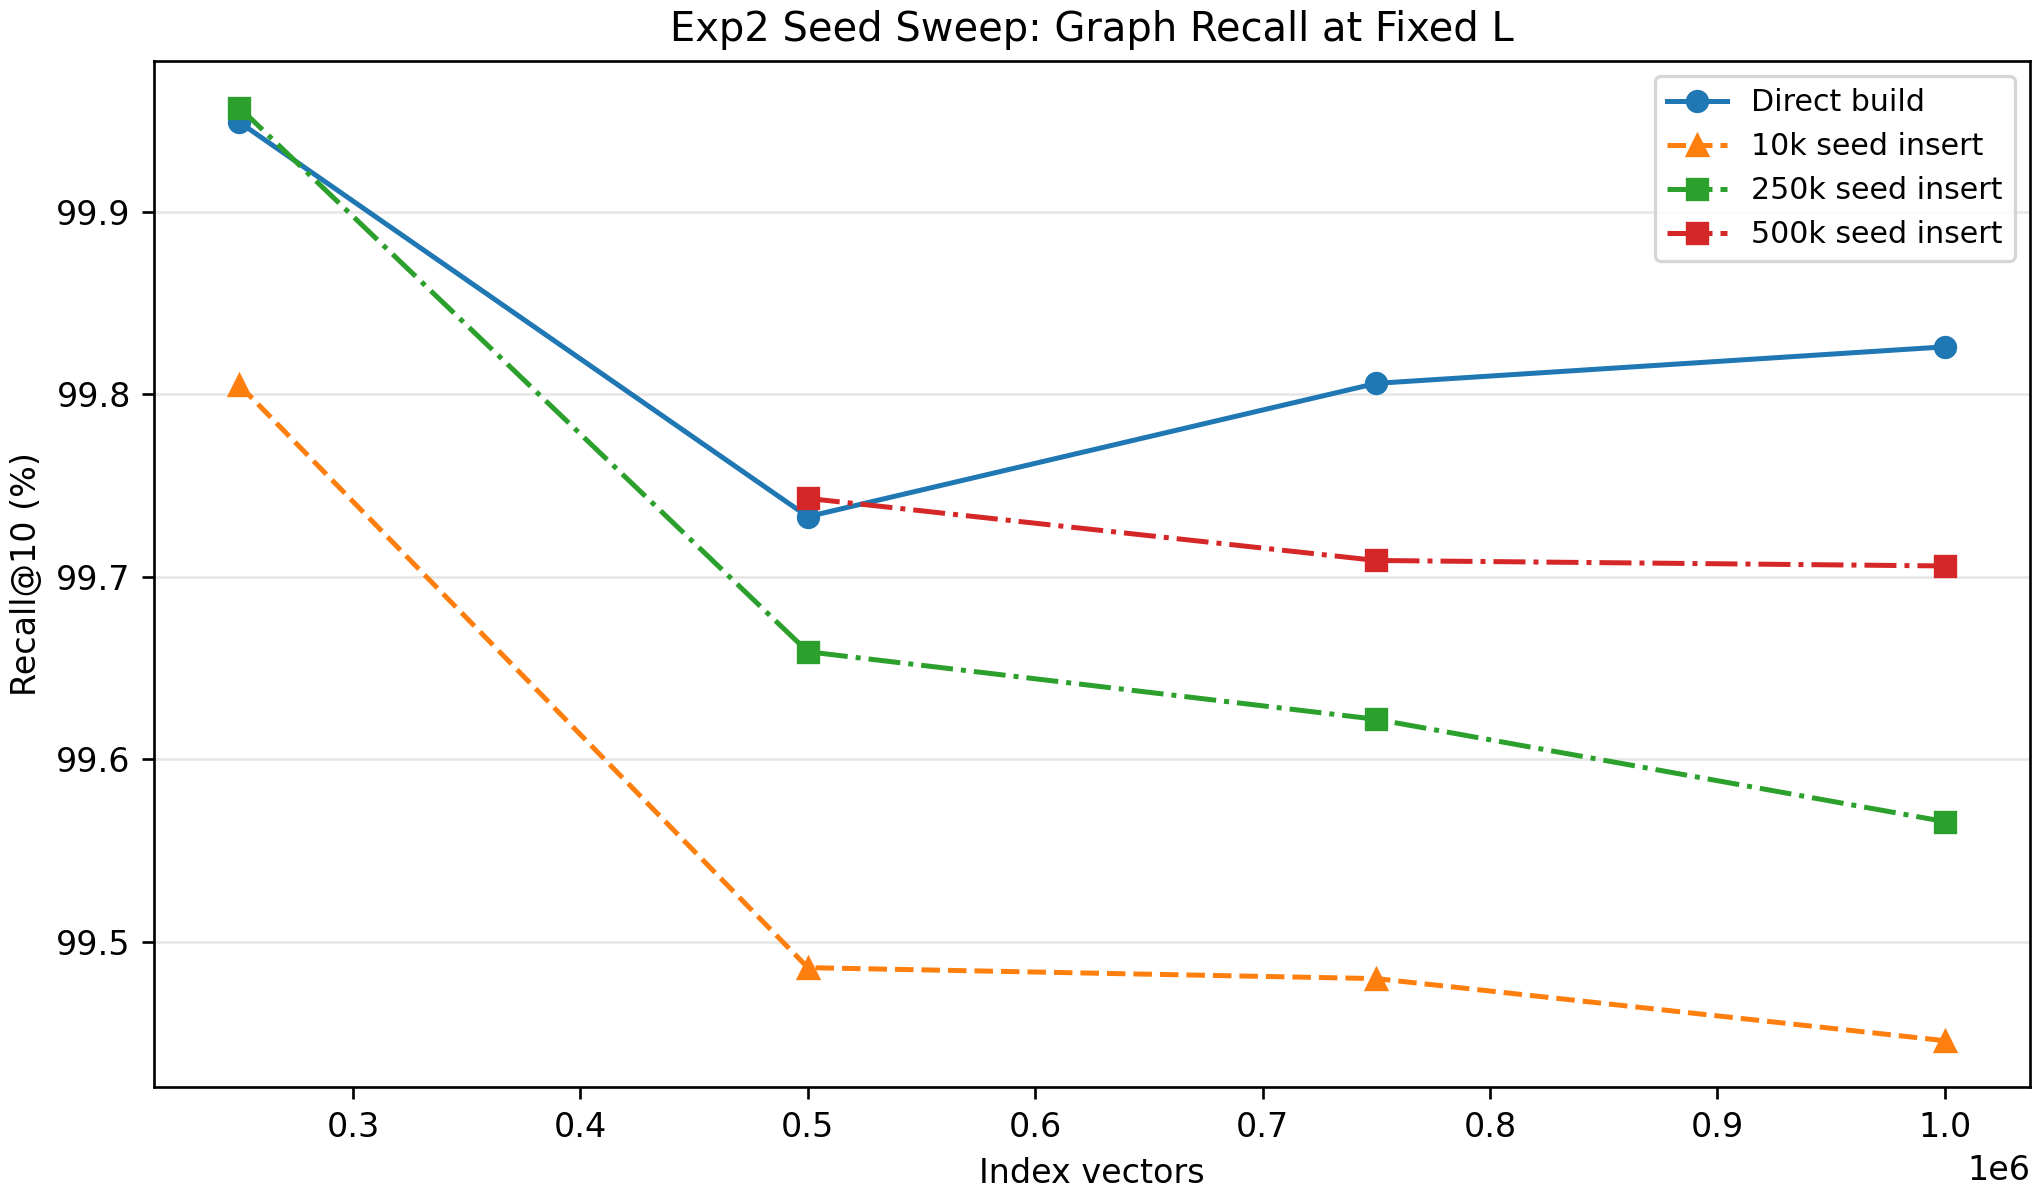
\includegraphics[width=0.98\linewidth,height=0.52\textheight,keepaspectratio]{../../experiments/r116_suite/exp2_stage_recall_build_vs_insert/seed_sweep_recall.png}

        \column{0.50\textwidth}
        \centering
        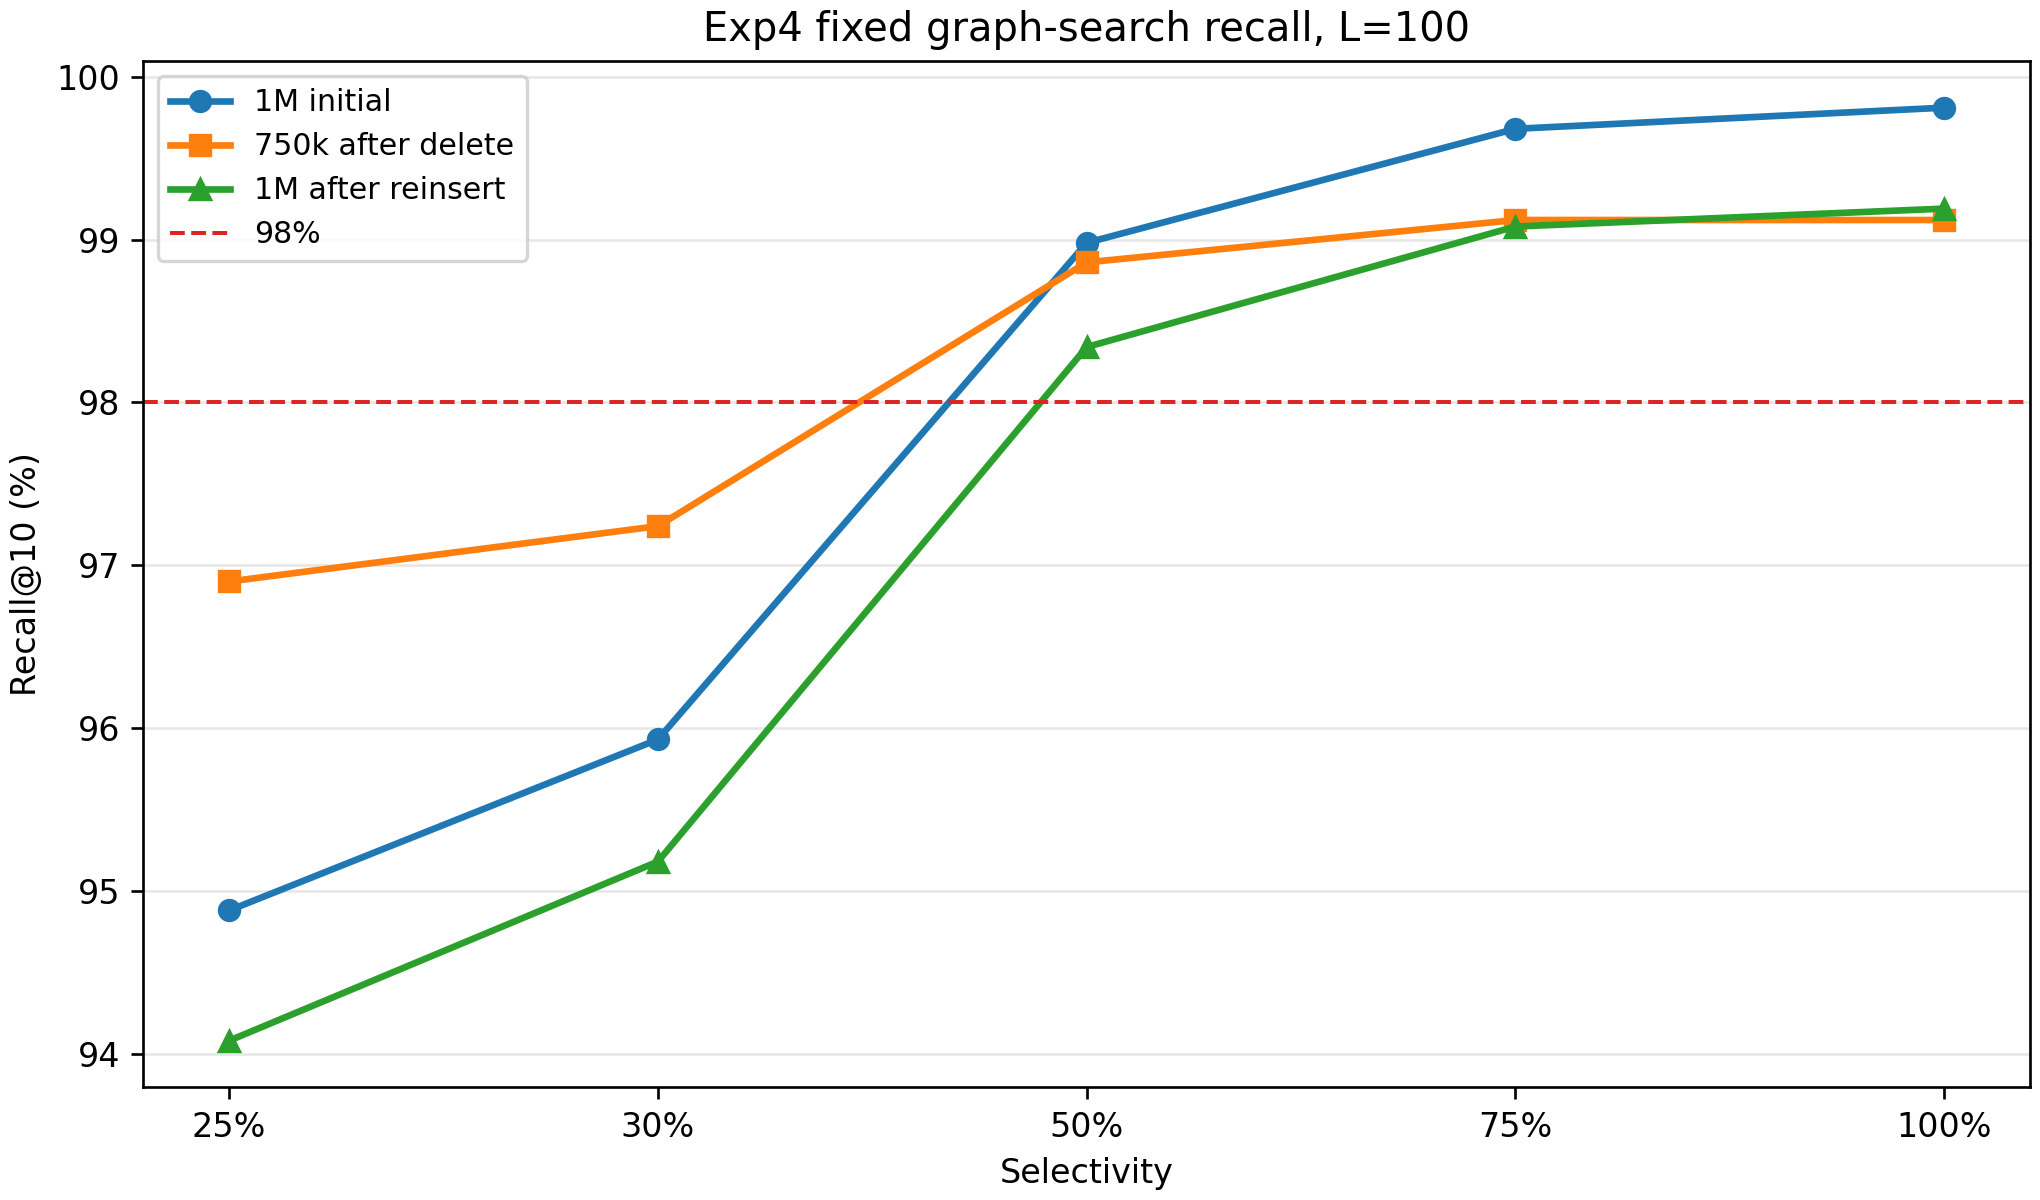
\includegraphics[width=0.98\linewidth,height=0.52\textheight,keepaspectratio]{../../experiments/r116_suite/exp4_delete_reinsert_selectivity/fixed_graph_recall_high_selectivity.png}
    \end{columns}
\end{frame}

\begin{frame}[c]{需求 2：插入期间前台查询}
    \centering
    \begin{minipage}{0.97\textwidth}
        \centering
        \small
        在初始 1M 索引上插入向量的同时执行前台搜索，测量搜索延迟与 QPS，结果如下图。

        \textcolor{red}{结论：在插入线程数小于 4 时，向量插入并不会对前台搜索性能产生显著影响。}
    \end{minipage}
    \vfill

    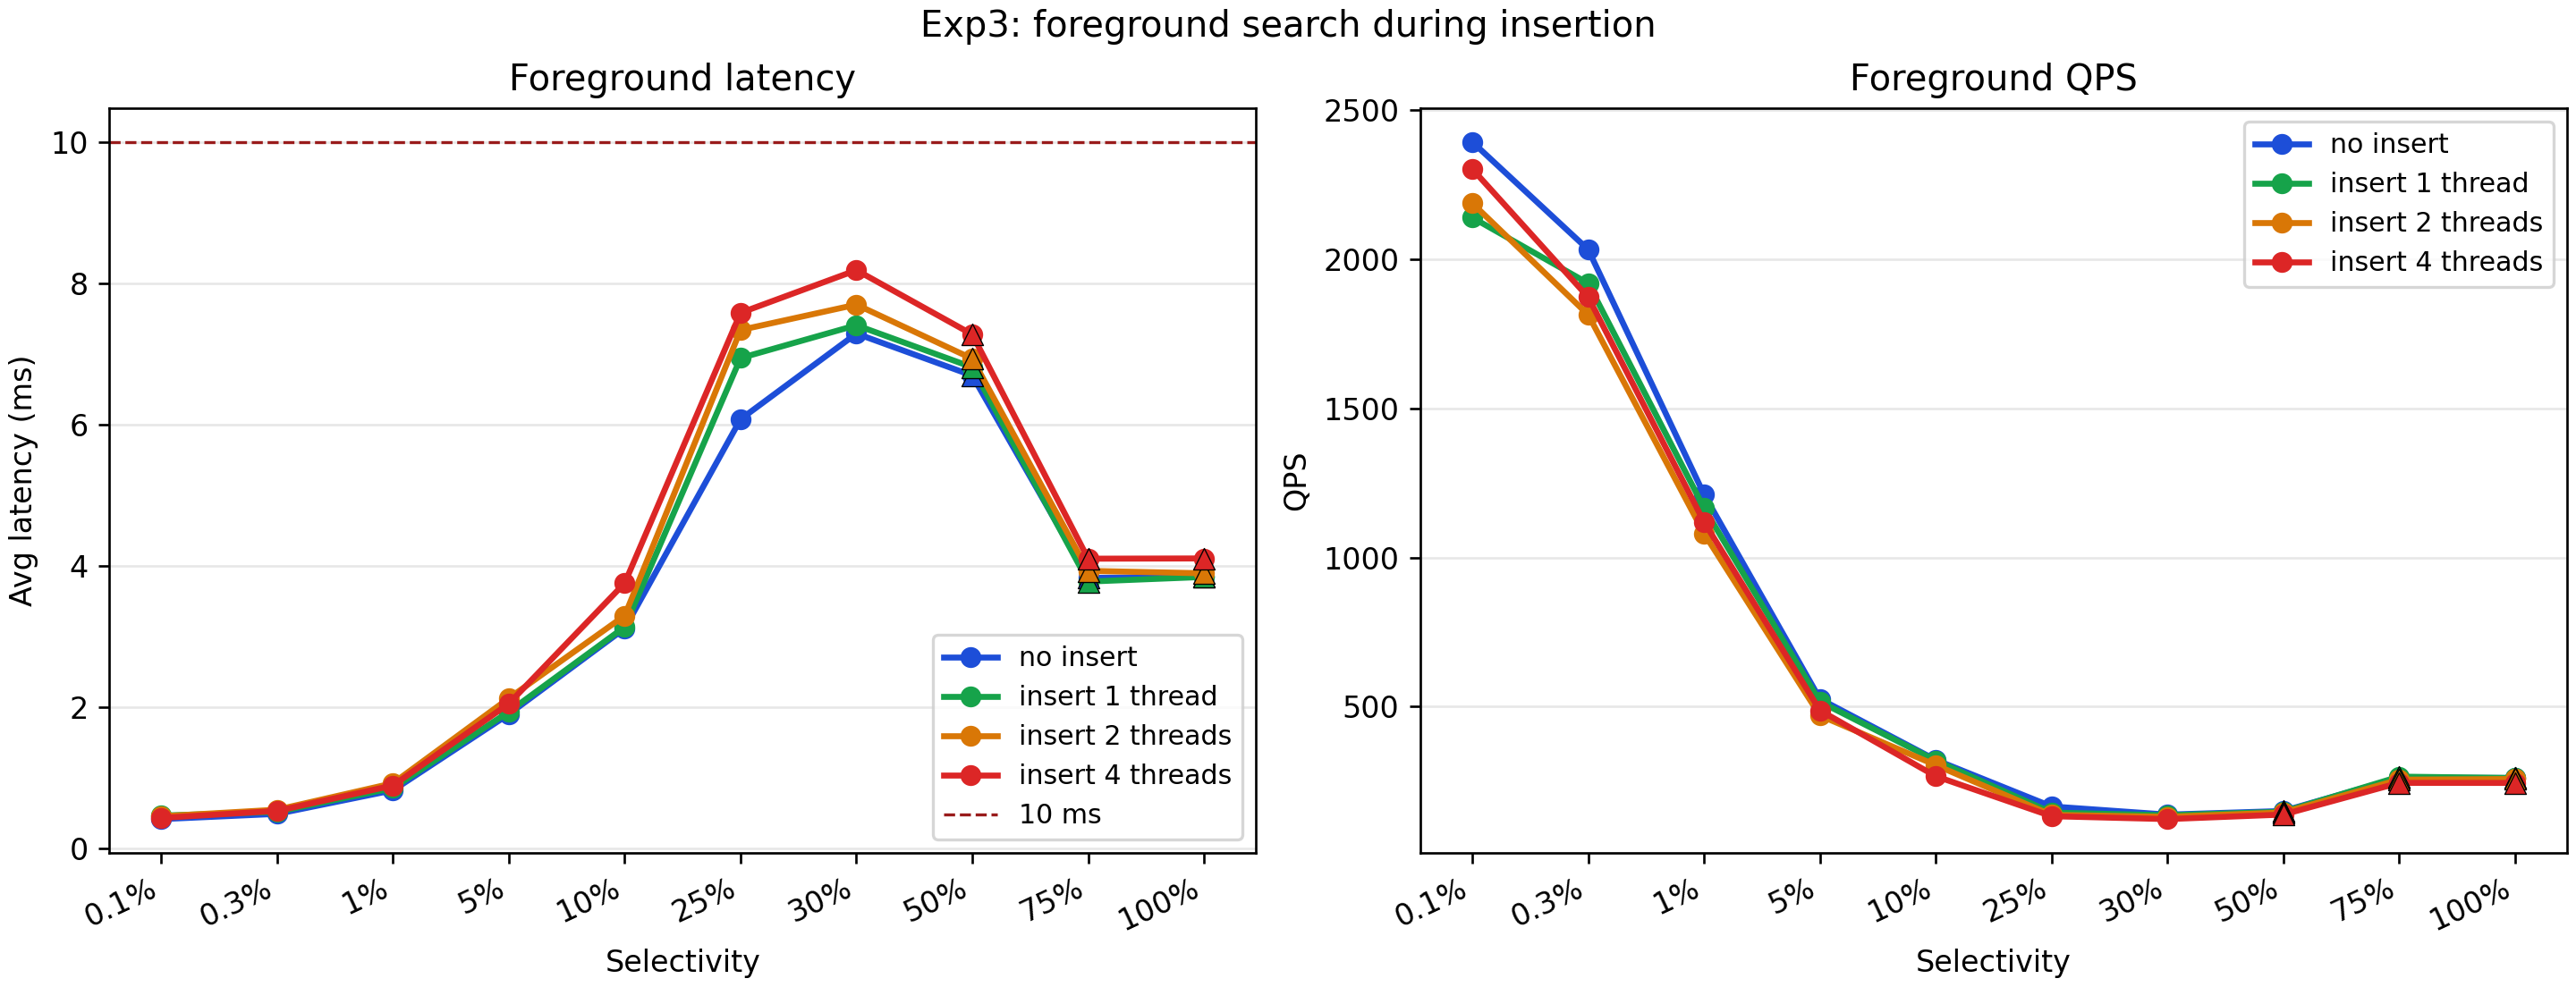
\includegraphics[width=0.94\linewidth,height=0.64\textheight,keepaspectratio]{../../experiments/r116_suite/exp3_search_during_insert/search_during_insert_selectivity.png}
\end{frame}

\begin{frame}[c]{需求 3：选择性查询延迟/QPS}
    \centering
    \begin{minipage}{0.94\textwidth}
        \centering
        \scriptsize
        在直接构建的 1M 索引上，对 intersect 等值过滤和 range 范围过滤分别校准 route/L，测量单线程 latency 与 QPS；本轮全量结果中所有点均满足 recall@10 $\geq$ 98。

        \textcolor{red}{结论：启用 io\_uring 后，intersect 与 range 全部选择性下单线程延迟均低于 10ms。}
    \end{minipage}
    \vfill

    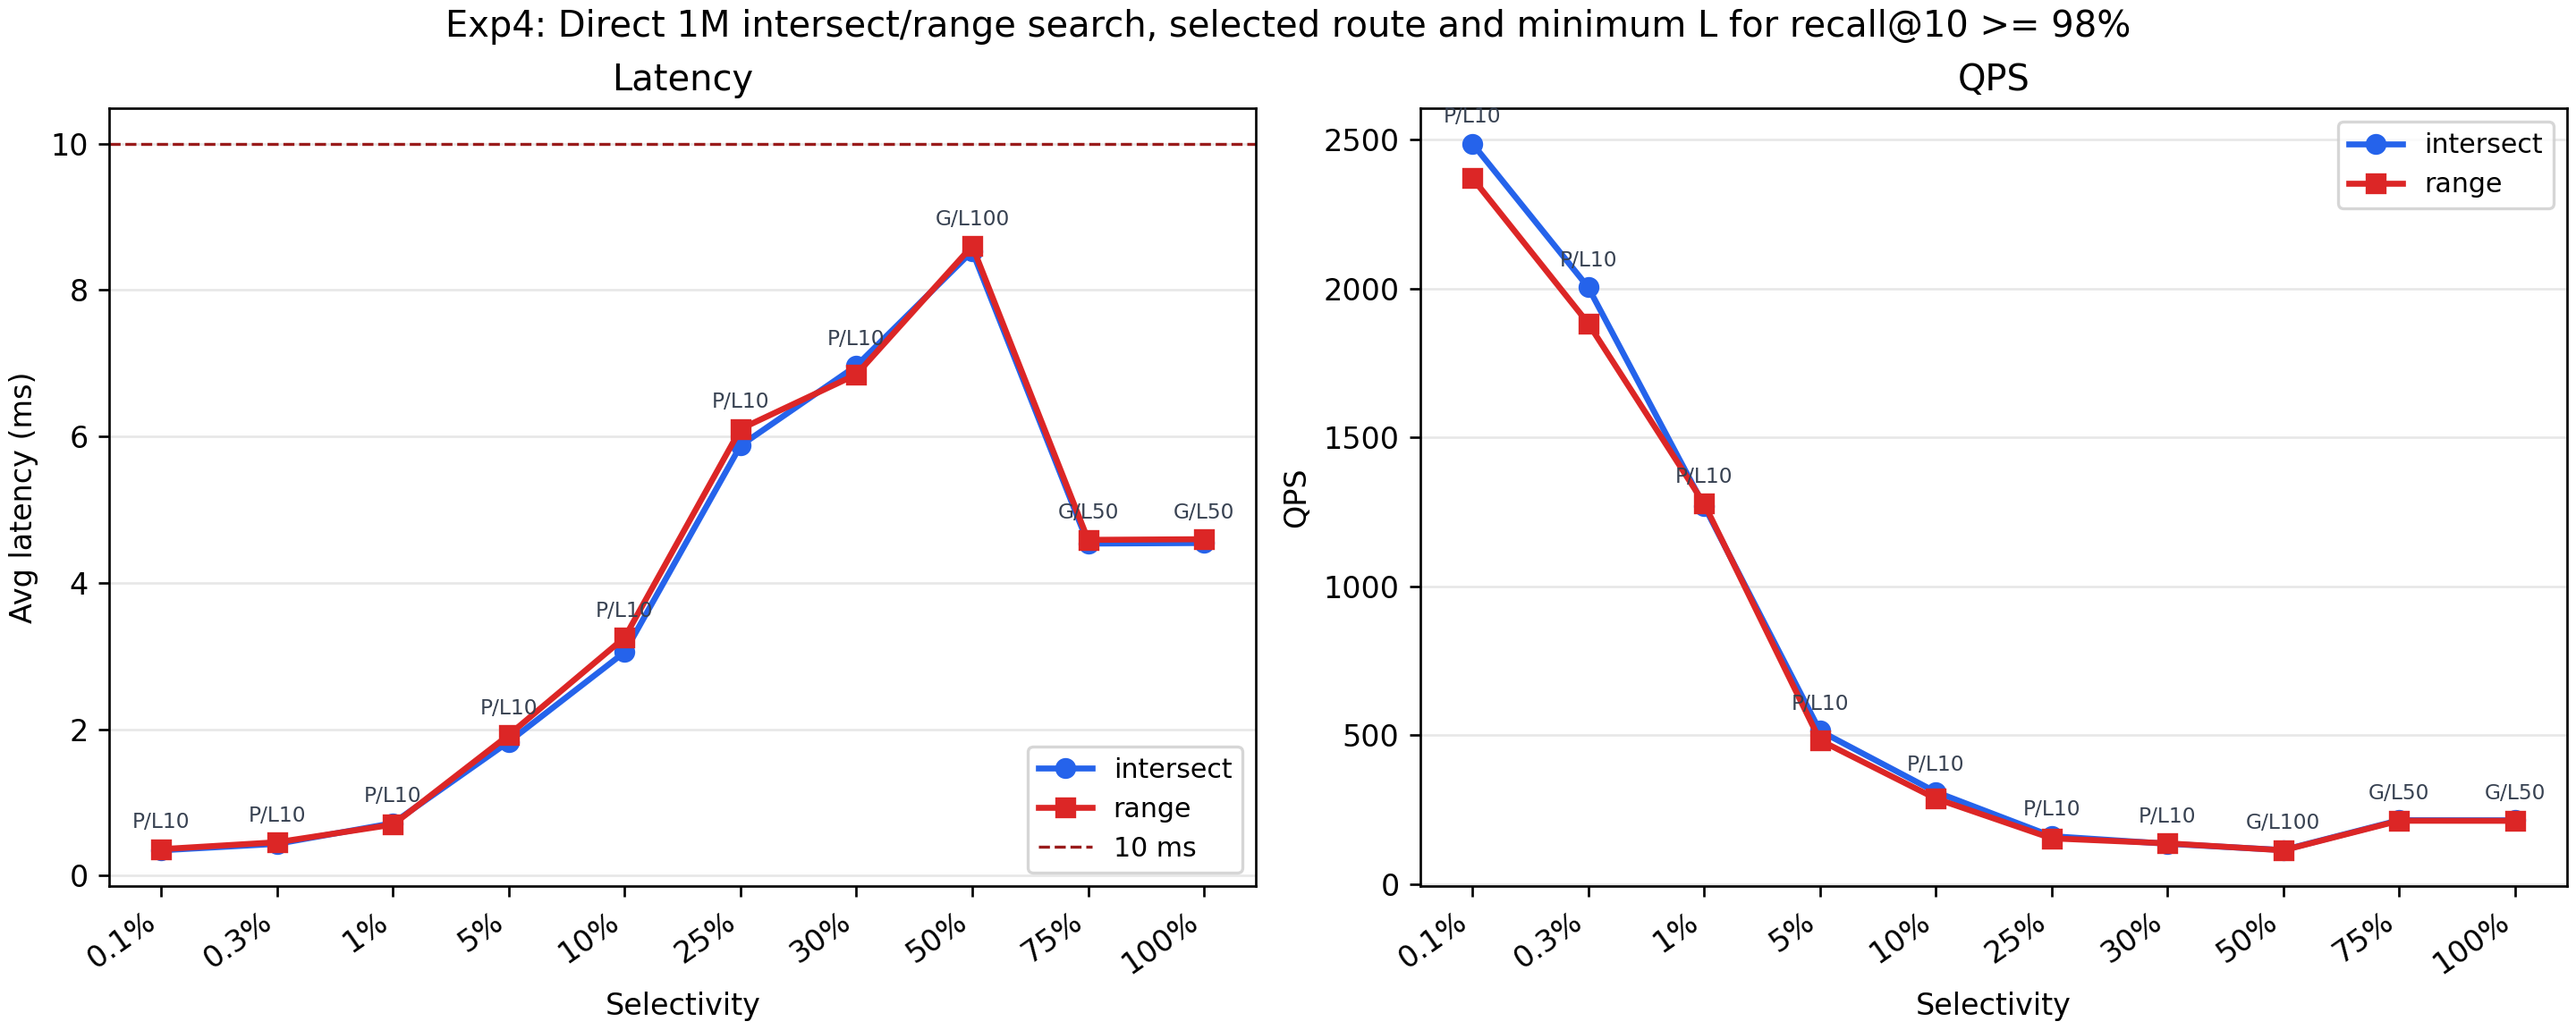
\includegraphics[width=0.94\linewidth,height=0.66\textheight,keepaspectratio]{../../experiments/r116_suite/exp4_intersect_range_selectivity/intersect_range_latency_qps.png}
\end{frame}

\begin{frame}[c]{需求 4：单查询 RSS}
    \centering
    \begin{columns}[c,onlytextwidth]
        \column{0.66\textwidth}
        \centering
        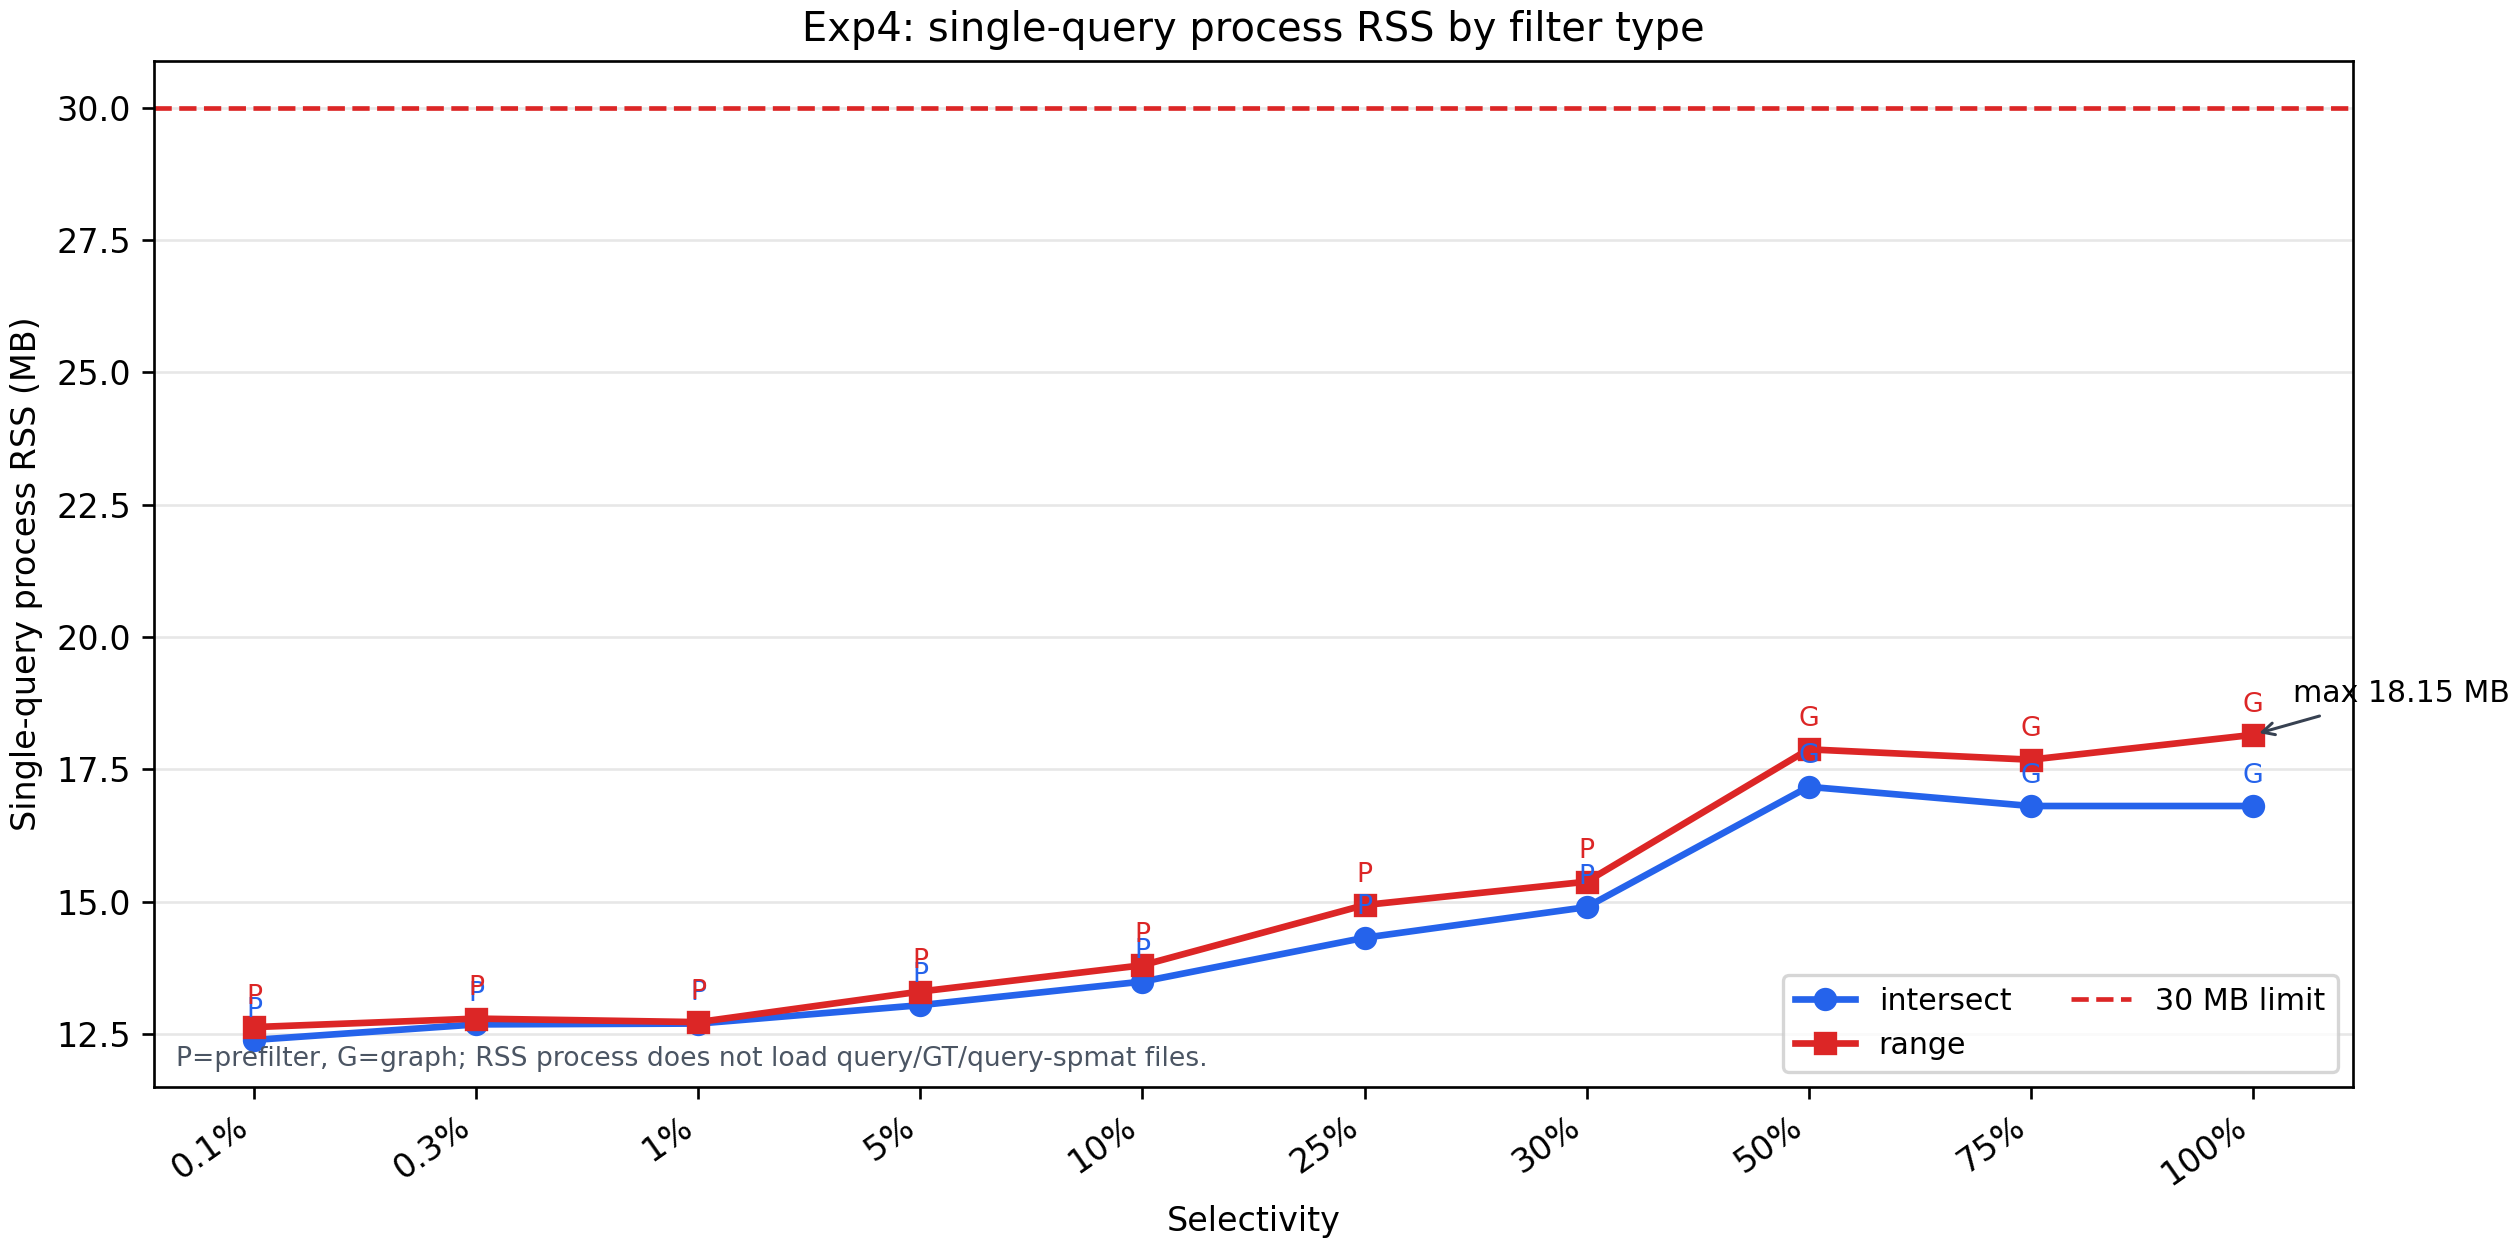
\includegraphics[width=0.98\linewidth,height=0.58\textheight,keepaspectratio]{../../experiments/r116_suite/exp4_intersect_range_selectivity/rss_by_selectivity.png}

        \column{0.32\textwidth}
        \centering
        \begin{minipage}{0.96\linewidth}
            \scriptsize
            \raggedright
            \textbf{口径}

            \vspace{0.25em}
            干净单查询进程总内存；query vector 和过滤 label 通过命令行传入，不加载 query file、groundtruth 或 query spmat。

            \vspace{0.25em}
            \textbf{实测结果}

            \vspace{0.25em}
            20 个点范围为 \textbf{12.39--18.15 MiB}；intersect 峰值 17.17 MiB，range 峰值 18.15 MiB。

            \vspace{0.25em}
            \textcolor{red}{结论：PQ code 改为 mmap 后，单查询进程 RSS 已低于 30MB 目标。}
        \end{minipage}
    \end{columns}
\end{frame}

\begin{frame}[c]{需求 5：索引空间组成}
    \centering
    \begin{minipage}{0.92\textwidth}
        \small
        原始向量空间按 \texttt{npoints * 128 * 4} 计算；额外索引空间均满足 extra/raw $\leq 1.0$。
        \vspace{0.5em}

        \scriptsize
        \begin{itemize}
            \item 250k：raw 122.07 MiB；其他文件合计 252.20 MiB，其中 disk.index 244.14 MiB，PQ compressed 7.63 MiB，PQ pivots 0.13 MiB，labels.densebit 0.30 MiB。
            \item 500k：raw 244.14 MiB；其他文件合计 504.27 MiB，其中 disk.index 488.29 MiB，PQ compressed 15.26 MiB，PQ pivots 0.13 MiB，labels.densebit 0.60 MiB。
            \item 750k：raw 366.21 MiB；其他文件合计 756.34 MiB，其中 disk.index 732.43 MiB，PQ compressed 22.89 MiB，PQ pivots 0.13 MiB，labels.densebit 0.89 MiB。
            \item 1M：raw 488.28 MiB；其他文件合计 1008.41 MiB，其中 disk.index 976.57 MiB，PQ compressed 30.52 MiB，PQ pivots 0.13 MiB，labels.densebit 1.19 MiB。
        \end{itemize}
    \end{minipage}
\end{frame}

\thanksforlistening{谢谢}

\end{document}
